\chapter{Introduction}\label{intro}
In this chapter we briefly discuss about motifs,what are they and why are we interested in them. Then we briefly describe the motif finding problem and various versions of it. We also give the formal description of the planted motif search for $ (l, d) $- motifs. Then we describe different approaches of motif searching algorithms and why we chose planted version of motif search. At the end of the chapter we give a short review of the mostly known approximate and exact PMS algorithm.


\section{What are Motifs}
Motif\index{Motif} means a pattern. A DNA motif is defined as a nucleic acid sequence that has some biological significance. By biological significance we mean it can be DNA binding sites for a regulatory protein that is a transcription factor. A DNA motif may be a small segment of nucleotide chain of A,T,C or G only 5 to 25 base pair long.

\subsection{Importance of Studying Motifs}
The discovery of rare event in DNA or protein sequence may lead new biological discoveries~\cite{dinh2012qpms7}. The presence of motifs is one kind of such rare events. Various biological processes such as gene expression may be controlled by motifs. Motifs are contained in regulatory regions of a genome such as promoters, enhancers, locus control regions etc~\cite{duret1997searching}. Generally, proteins known as transcription factors regulate the expression of a gene by binding to locations of motifs in regulatory regions. For example transcription factors such as TFIID, TFIIA and TFIIB usually bind to sequence 5'-TATAAA-3' in the promoter region of a gene in order to initiate its transcription. Such motifs and their locations in regulatory regions like binding sites are important and helpful to uncover the regulatory mechanism of gene expression which is very sophisticated. Motif search also has many applications in solving some crucial biological problems. For example, finding motifs in DNA sequences is very important for the determination of open reading frames, identification of gene promoter elements, location of RNA degradation signals and the identification of alternative splicing sites~\cite{pal2016efficient}.
In protein sequences, patterns have led to domain identification, location of protease cleavage sites, identification of signal peptides, protein interactions, determination of protein degradation elements, identification of protein trafficking elements etc.  So we can agree to the fact that, motif identification plays an important role in biological studies.

\subsection{Regulatory Regions and Transcription Factor Binding Sites}
DNA regions involved in transcription and transcriptional regulation are called regulatory regions (RR). Every gene contains a RR typically stretching 100-1000 bp
upstream of the transcriptional start site. A transcription factor (TF) is a protein that can bind to DNA and regulate gene expression. TFs influence gene expression by binding to a specific location in the respective genes regulatory region which is known as TFBSs or motifs. TFBSs are a part of either the promoter or enhancer region of a gene.

\section{The Motif Finding Problem}
Our target is to identify transcription factor binding sites or motif from a DNA sequence. We are given a set of DNA sequences of specified length and the length of the motif. We choose a position from every sequence which will be the starting sequence for the motif candidates \Cref{fig:sindex}. Taking these sequences we make alignment matrix, profile matrix and finally consensus string. Then we evaluate the consensus string with the help of a scoring function. Now, we have to find the starting position for which the score of the consensus string will be maximum. It is the informal description of the motif searching problem. 

\begin{figure}%[H]
	\centering
	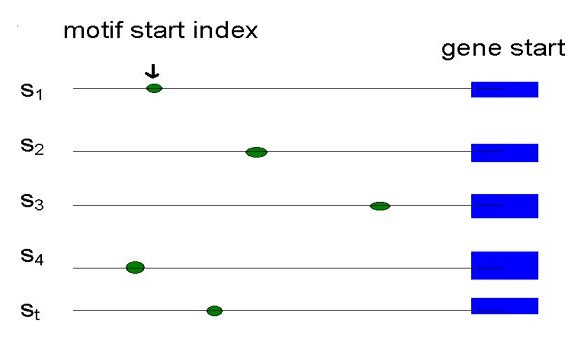
\includegraphics[width=0.6\textwidth]{figures/sindex}
	\caption{Starting index of motifs in a DNA sequence .}
	\label{fig:sindex}
\end{figure}

\subsection{Classification of Motif Searching Algorithms}
For the importance of motifs, various motif finding algorithms have been researched and applied for the last two decades. We can classify these algorithms in to three categories. All motif searching algorithms follow one of the three approaches:
\begin{itemize}
	\item \textbf{Combinatorial Approach :} Tries to explore exhaustively all the ways that a molecular process could happen thus leads to hard combinatorial problems for which efficient algorithms are required.
	\item \textbf{Probabilistic Approach :} Makes certain decisions randomly by extending the classical model of deterministic algorithms. They are often faster, simpler and more elegant than their	combinatorial counterparts. 
	\item \textbf{Phylogenetic Footprinting Approach :} Discovers regulatory elements in a set of orthologous regulatory regions from multiple species by identifying the best
	conserved motifs in those orthologous regions.
\end{itemize}

\subsection{Combinatorial Approach}
Among the various approaches combinatorial approach that has proven to be more accurate than the others. In our approach we will use combinatorial algorithms for the discovery of motifs. The are several versions of this approach. Mosty used three versions are:
\begin{itemize}
	\item Planted Motif Search (PMS)
	\item Simple Motif Search (SMS)
	\item Edited-distance-based Motif Search (EMS)~\cite{rajasekaran20091}
\end{itemize}

\subsection{Planted Motif Search (PMS)}\index{Planted Motif Search}
Among different versions of combinatorial approaches the PMS problem is more popular due to its closeness to motif reality.  Motifs typically occur with mutations at binding sites. The binding sites are referred to as instances of a motif. A motif in PMS is referred to as a $ (l, d) $-motif where $ l $ is its length and $ d $ is the
maximum number of mutations allowed for its instances. Given a set of n sequences, the PMS Algorithm tries to find all the $ (l, d) $-motifs in them. The PMS problem is essentially the same as the closest substring problem.

\subsection{Quorum Planted Motif Search (qPMS)}
A generalized version of the PMS Problem namely Quorum Planted Motif Search (qPMS) problem\index{Quorum Planted Motif Search}. The qPMS problem is to find all the motifs that have motif instances present in $ q $ out of the $ n $ input sequences. This version captures the nature of motifs more precisely than the PMS problem because in practice some motifs may not have motif instances in all of the input sequences. qPMS algorithms can be used to find DNA motifs and protein motifs as well as transcription factor binding sites. 

\subsection{Formal Definitions of qPMS}
\qquad \textbf{Definition 1 } A string $ x=x[1]\dots x[l] $ of length $ l $ is called an $ l $-mer. 

\qquad \textbf{Definition 2 } Given two strings $ x=x[1]\dots x[l] $ and $ s=s[1]\dots s[m] $ with $ l<m $ we say $ x\epsilon_{l}s $ if there exists $ 1\leq i \leq l-m+1 $ such that $ x[j]=s[l-m+1] $ for every $ 1\leq j\leq l $. We also say that $ x $ is an $ l $-mer in $ s $.

\qquad \textbf{Definition 3 } Given two strings $ x=x[1]\dots x[l] $ and $ y=y[1]\dots y[l] $ of equal length, the Hamming distance between $ x $ and $ y $ denoted by $ d_{H}(x,y) $ is the number of mismatches between them. In other words, $ d_{H}(x,y)=\Sigma_{1\leq i \leq l}I_{i} $, where $ I_{i} $ is the indicator at position $ i $. $ I_{i}=1 $ if $ x[i]\neq y[i] $ and $ I_{i}=0 $ otherwise.

\qquad \textbf{Definition 4 } Given two strings $ x $ and $ s $ with $ |x|<|s| $, the Hamming distance between $ x $ and $ s $, denoted by $ d_{H}(x,s) $ is $ \min _{y\epsilon _{|x|}s} d_{H}(x,y) $.

\qquad \textbf{Definition 5 } Given a set of $ n $ strings $ s_{1},\dots,s_{n} $ of length $ m $ each, a string $ M $ of length $ l $ is called an $ (l, d, q) $-motif of the strings if there are at least $ q $ out of the $ n $ strings such that the Hamming distance between each one of them and $ M $ is no more than $ d $.

\qquad \textbf{Definition qPMS } Given $ n $ input strings $ s_{1},\dots,s_{n} $ of length $ m $ each, three integer parameters $ l $, $ d $ and $ q $, find all the $ (l,d,q) $-motifs of the input strings. The PMS problem is a special case of the qPMS problem when $ q=n $.

\section{Literature Review}
During the last two decades various types of PMS algorithm has been proposed in the literature. There are mainly two types of algorithms for PMS problem. They are \textit{exact} and \textit{approximate} algorithms. An exact algorithm always finds all
the $ (l, d) $-motifs present in the input sequences. While, an approximate algorithm may not find all the motifs. 

\subsection{Exact PMS Algorithms}
An exact algorithm can find all the motifs in input sequences. In our research paper, we only consider exact algorithms. The exact variant of the PMS problem has been shown to be NP-hard~\cite{frances1997covering}. It means that there is no PMS algorithm that takes only polynomial time to iterate. As a result, all known exact algorithms have an exponential worst case runtime. Due to NP-hardness approximate algorithm arises for PMS. An exact PMS algorithm can be built using two approaches:

\subsubsection{Sample Driven Approach}\index{Sample Driven}
For all $ (m - l + 1)^{n} $ possible combinations of $ l $-mers coming from different strings generate the common neighborhood. Unlike pattern driven approach in \textit{Sample Driven (SD)} approaches all possible motifs generated from the $ l $-mers in input strings are of interest which could be found in polynomial time. \textit{Sample Driven} algorithms try to find comparative patterns by comparing the given length strings and looking for
local similarities between them. They are based on constructing a local multiple alignment of the given non-coding DNA sequences and then extracting the comparative patterns from the alignment by combining the segments which is common to most of the
non-coding DNA sequences.

\subsubsection{Pattern Driven Approach}\index{Pattern Driven}
For all $ |\Sigma|^{l} $ possible $ l $-mers check which are motifs. Trying all possible motif candidates take exponential space. \textit{Pattern Driven (PD)} algorithms are based on enumerating candidate patterns in a given length string and inputting substrings with high fitness. Compared with \textit{SD} algorithms, \textit{PD} algorithms can be performed intelligently so that patterns are not present in the data that are not generated.


All existing exact algorithms solve PMS problem in exponential time in some of its parameters. The most recent exact algorithms that have been proposed in the literature are Algorithm \textit{qPMS9} due to ~\cite{nicolae2015qpms9}, Algorithm \textit{PMS8} due to ~\cite{nicolae2014efficient}, Algorithm \textit{Pampa} due to ~\cite{davila2007pampa}, Algorithm \textit{qPMS7} due to ~\cite{dinh2012qpms7}, Algorithm \textit{PMSPrune} due to ~\cite{davila2007fast}, Algorithm \textit{PMS6} due to ~\cite{bandyopadhyay2013pms6mc}, Algorithm \textit{Voting} due to ~\cite{chin2005voting}, and Algorithm \textit{RISSOTO} due to ~\cite{pisanti2006risotto}.


\subsection{Approximate PMS Algorithms}
Approximate PMS algorithms usually tend to be faster than exact PMS algorithms. Typically, approximate PMS algorithms employ heuristics such as local search, Gibbs sampling, expectation optimization etc. Some examples of approximate algorithms are Algorithm \textit{MEME} due to ~\cite{bailey1994fitting}, Algorithm \textit{PROJECTION} due to ~\cite{buhler2002finding}, Algorithm \textit{Gibbs DNA} due to ~\cite{lawrence1993detecting}, Algorithm \textit{WINNOWER} due to ~\cite{pevzner2000combinatorial}, and Algorithm \textit{Random Projection} due to ~\cite{rocke1998algorithm}. Some other approximate PMS algorithms are Algorithm \textit{MULTIPROFILER} due to ~\cite{keich2002finding}, Algorithm \textit{PatternBranching} due to ~\cite{price2003finding} and Algorithm \textit{CONSENSUS} due to ~\cite{hertz1999identifying}.

\subsubsection{Algorithm MEME}\index{Algorithm!MEME}
The MEME algorithm extends the EM algorithm for identifying motifs in unaligned sequences. While a drawback of EM is that the maximum it finds is only local, MEME can either favor motifs that appear exactly once or appear zero or once in each sequence in a training set, or give no preference to a number of occurrences. In 2005 \textit{Hall et al} acquired a set of correlated genes from genomic, transcriptomic and proteomic analyses. They applied MEME to scan 1000 bp of the 3' end of stop codon, where a 47 bp motif was found in six of the analyzed sequences. Then it was used to search the entire genome and 20 additional genes were identified to have the same motif. This motif was known to be bound to Puf protein, implying that Puf protein may control the transcription of the analyzed genes.

\subsubsection{Algorithm Projection}\index{Algorithm!Projection}
This algorithm ameliorates the limitations of existing algorithms by using random projections of input. It extends previous projection-based searching techniques to solve a multiple alignment problem that is not effectively addressed by pairwise alignments. It is designed to efficiently solve the problems from the planted $ (l, d) $-motif model and can do more reliably and substantially difficult instances than previous algorithms. For $ t= 20 $ and $ n= 600 $ this algorithm achieves performance close to the best possible, being limited primarily by statistical considerations.

\subsubsection{Algorithm Winnower, SP-STAR, and cWinnower}\index{Algorithm!Winnower}
Winnower first represents motif instances as vertices then it tries to delete spurious edges and recover motifs with the remaining vertices. SP-STAR is a local sum of pairwise score improvement algorithm which considers only the subsequences present in dataset and iteratively updates scores of the motifs. cWinnower improves its running time by a stronger constraint function.



\endinput

%See these examples:
%\begin{itemize}
%	\item 
%	\item \Cref{fig:sample} is a sample figure.
%	\item \Cref{tab_our} is a table.
%	\item \Cref{sec:cite} in \Cref{ch:citations} shows some examples of
%	  citations.
%\end{itemize}

%\section{How to Write a Section}
%
%This is for writing section.
%
%\section{How to Add Table and Figures}\label{contribution}
%You should refer a figure as, ``\Cref{fig:sample} is a sample
%figure''.
%
%\begin{figure}[!tb]
%  \centering
%  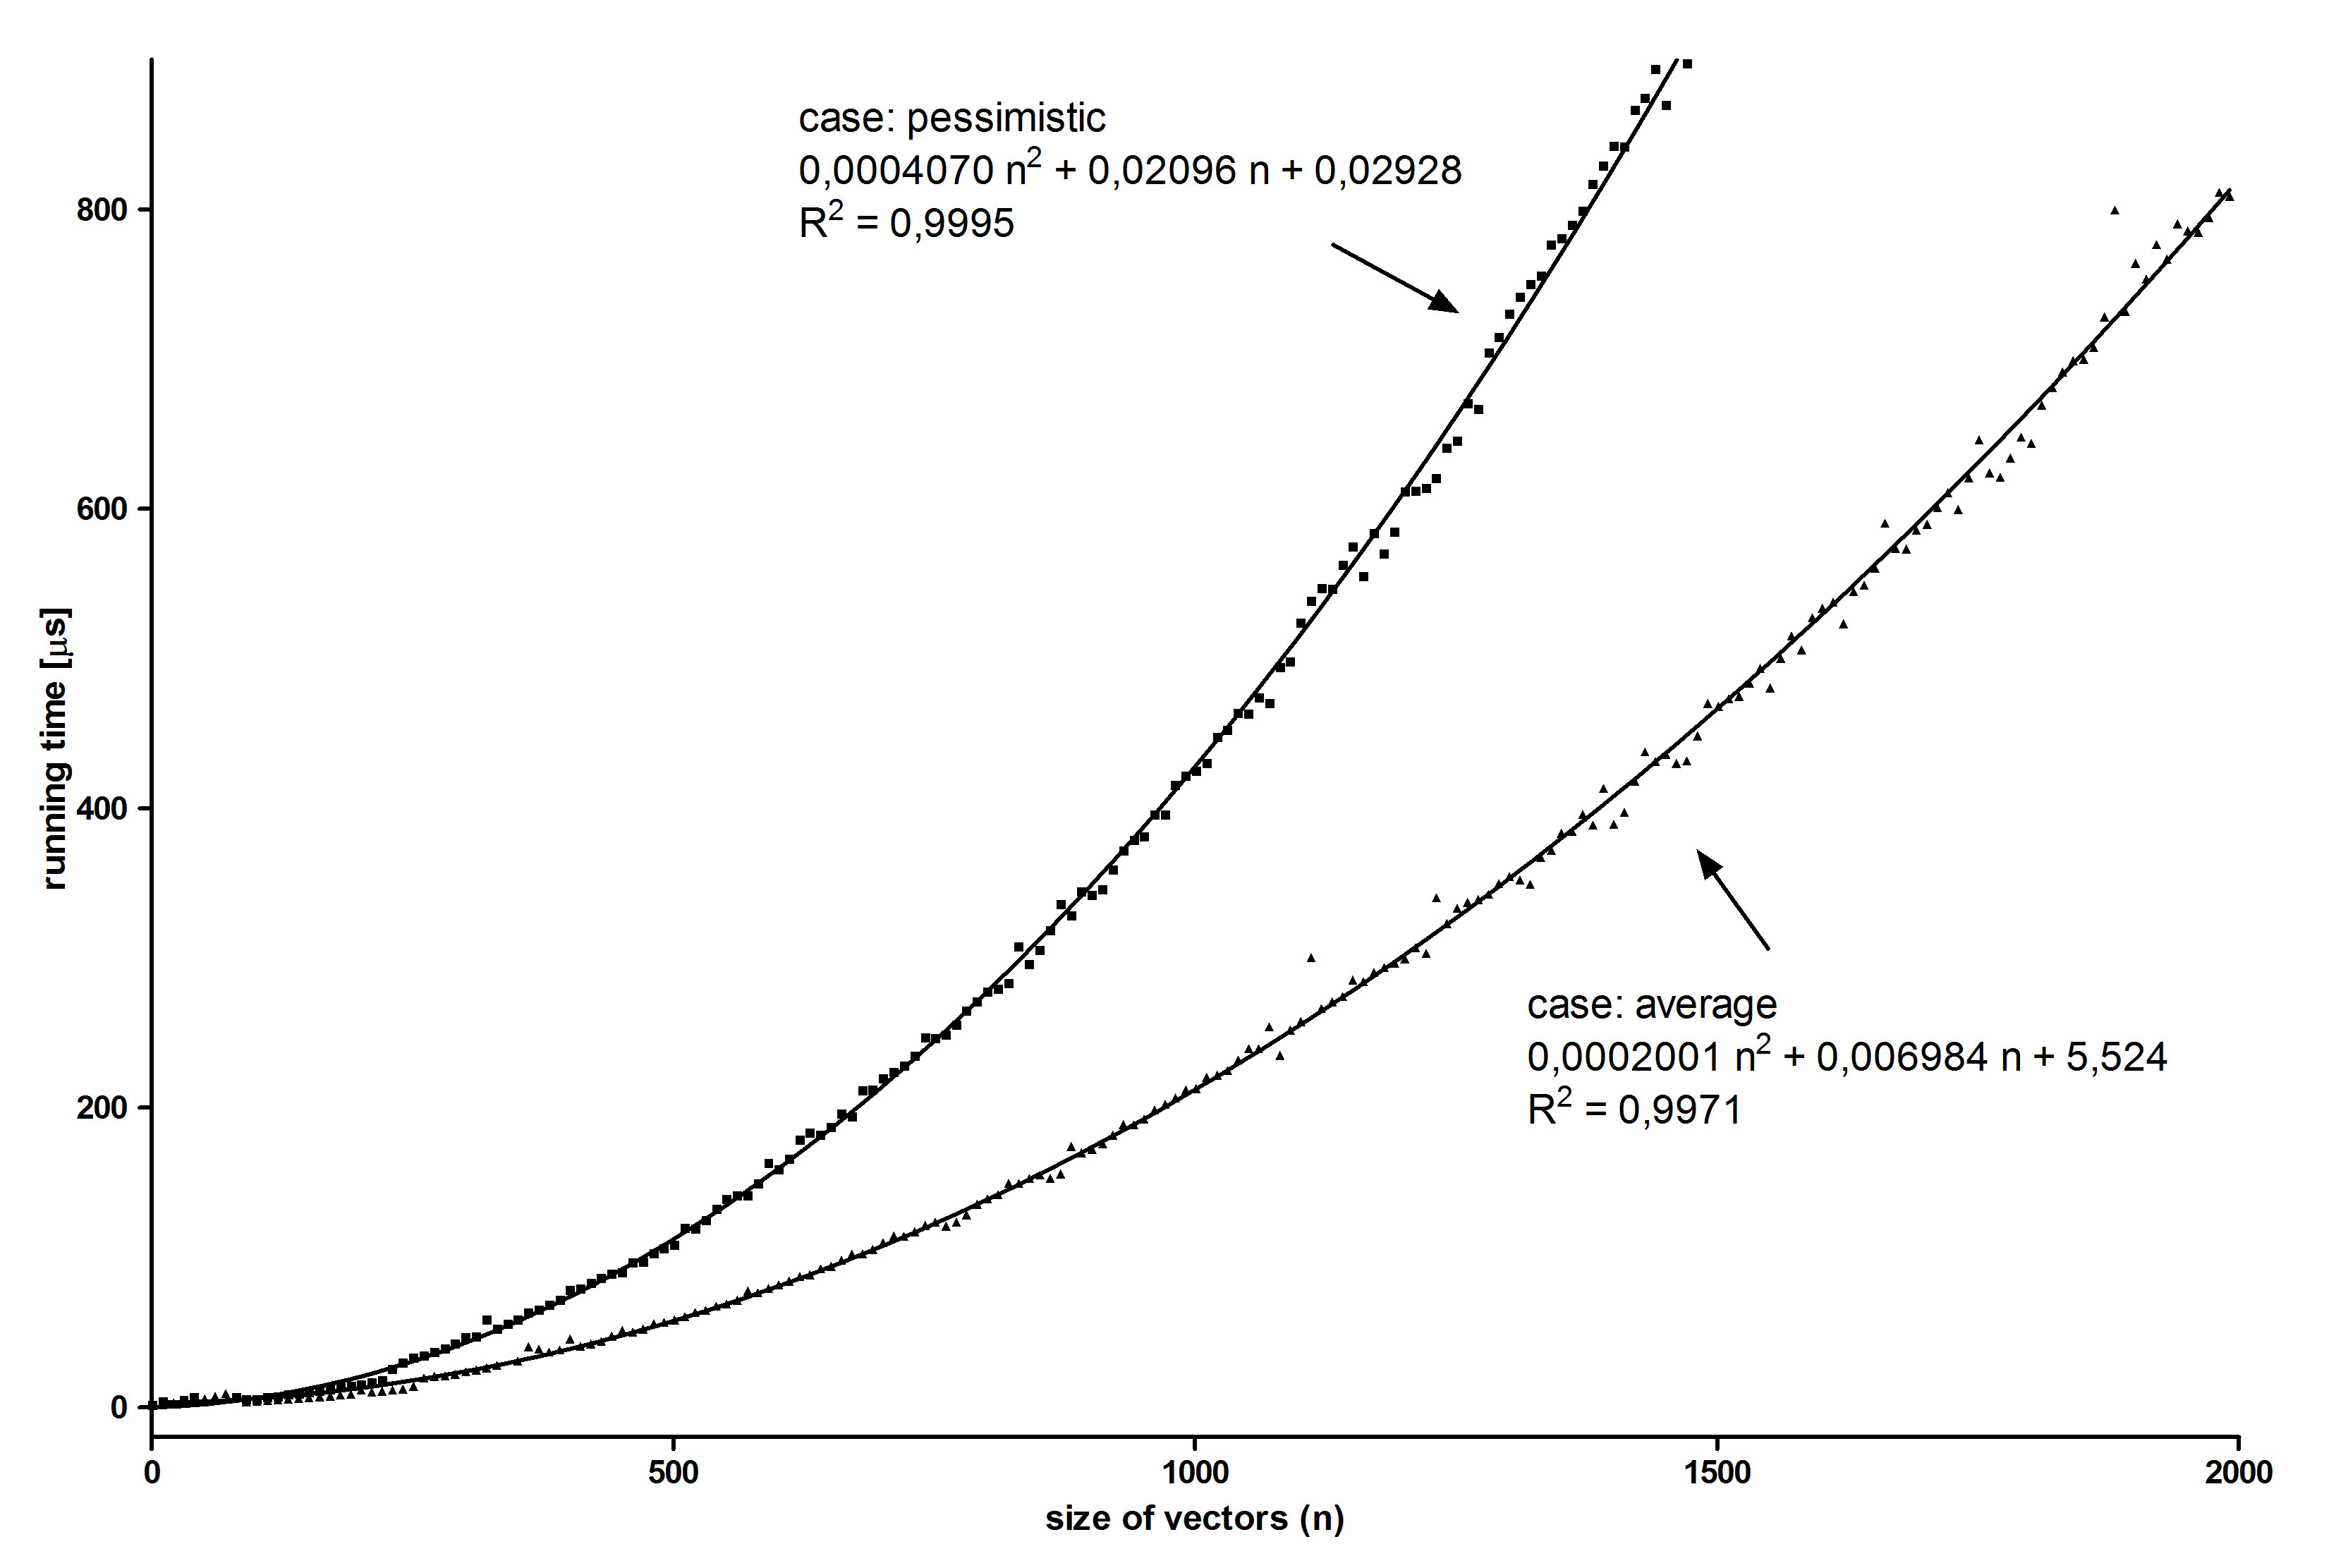
\includegraphics[width=0.9\textwidth]{figures/sample}
%  \caption{This is a sample figure.}
%  \label{fig:sample}
%\end{figure}
%
%				
%Then we applied same test cases to our modified algorithm i.e.\ the
%heuristic algorithm with our new operation \textit{Block Reversal}. The
%performance is shown in \Cref{tab_our}.


%\begin{table}[!tb]
%  \begin{center}
%    \caption{Performance table of \emph{Block reversal} in a heuristic algorithm ($n=20$)}
%    \label{tab_our}
%
%    \begin{tabular}{|l|r|r|r|r|r|r|r|r|r|r|r|r|r|}
%      \hline
%      $\alpha$     & $\alpha n$ & \multicolumn{11}{c|}{Test Cases} & \multicolumn{1}{c|}{Average \# of}                                     \\
%      \cline{3-13} &            & 1                                & 2  & 3  & 4  & 5  & 6  & 7  & 8  & 9  & 10 & 11 & calculated operation \\
%      \hline
%      0.1        & 2          & 2                                & 2	& 2  & 2  & 2  & 2  & 2  & 2  &	2  & 2	& 2  & 2                    \\
%      0.2        & 4          & 4                                & 4	& 5  & 2  & 4  & 4  & 4  & 4  &	2  & 4	& 4  & 3.73                 \\
%      0.3        & 6          & 5                                & 6	& 6  & 6  & 6  & 7  & 6  & 5  &	6  & 6	& 6  & 5.91                 \\
%      0.4        & 8          & 7                                & 8	& 5  & 6  & 7  & 6  & 6  & 7  &	8  & 8	& 7  & 6.82                 \\
%      0.5        & 10         & 9                                & 10	& 6  & 12 & 10 & 8  & 10 & 10 &	7  & 7	& 10 & 9                    \\
%      0.6        & 12         & 9                                & 12	& 16 & 10 & 12 & 12 & 9  & 11 &	12 & 9	& 12 & 11.27                \\
%      0.7        & 14         & 13                               & 7	& 18 & 15 & 14 & 8  & 13 & 11 &	13 & 13	& 14 & 12.64                \\
%      0.8        & 16         & 10                               & 17	& 14 & 16 & 13 & 16 & 13 & 11 &	13 & 17	& 13 & 13.91                \\
%      0.9        & 18         & 14                               & 16	& 15 & 12 & 15 & 11 & 15 & 11 &	15 & 12	& 12 & 13.45                \\
%      1          & 20         & 18                               & 11	& 13 & 11 & 13 & 15 & 17 & 17 &	13 & 18	& 12 & 14.36                \\
%      \hline
%    \end{tabular}
%  \end{center}
%\end{table}
%

